

\section{Tutorial Problem}
\tbd{Update according new scheme or rather generate from commented YAML input file.}
In the following section, we shall provide an example cook book for preparing and running a model. It is 
one of the test problem with the main input file:
\begin{verbatim}
tests/03_transport_small_12d/flow_vtk.con
\end{verbatim}
We shall start with preparation of the geometry using an external software and then we shall go thoroughly through the 
commented main input file. The problem includes steady Darcy flow, transport of two substances with explicit
time discretization and a reaction term consisting of dual porosity and sorption model.

\subsection{Geometry}
We consider a~simple 2D problem with a branching 1D fracture (see Figure \ref{fig:tutorial} for the geometry). 
To prepare a~mesh file we use the \href{http://geuz.org/gmsh/}{GMSH software}.
First, we construct a~geometry file. In our case the geometry consists of: 
\begin{itemize}
 \item one physical 2D domain corresponding to the whole square
 \item three 1D physical domains of the fracture
 \item four 1D boundary physical domains of the 2D domain
 \item three 0D boundary physical domains of the 1D domain
\end{itemize}
In this simple example, we can in fact combine physical domains in every group, however we use this more complex setting for
demonstration purposes. Using GMSH graphical interface we can prepare the GEO file where physical domains are referenced by numbers, then we use 
any text editor and replace numbers with string labels in such a way that the labels of boundary physical domains start with the dot character. 
These are the domains where we will not do any calculations but we will use them for setting boundary conditions.
Finally, we get the GEO file like this:

\begin{multicols}{2}
{\small
\begin{Verbatim}[numbers=left]
cl1 = 0.16;
Point(1) = {0, 1, 0, cl1};
Point(2) = {1, 1, 0, cl1};
Point(3) = {1, 0, 0, cl1};
Point(4) = {0, 0, 0, cl1};
Point(6) = {0.25, -0, 0, cl1};
Point(7) = {0, 0.25, 0, cl1};
Point(8) = {0.5, 0.5, -0, cl1};
Point(9) = {0.75, 1, 0, cl1};
Line(19) = {9, 8};
Line(20) = {7, 8};
Line(21) = {8, 6};
Line(22) = {2, 3};
Line(23) = {2, 9};
Line(24) = {9, 1};
Line(25) = {1, 7};
Line(26) = {7, 4};
Line(27) = {4, 6};
Line(28) = {6, 3};
\end{Verbatim}
\columnbreak
\begin{Verbatim}[numbers=left, firstnumber=last]
Line Loop(30) = {20, -19, 24, 25};
Plane Surface(30) = {30};
Line Loop(32) = {23, 19, 21, 28, -22};
Plane Surface(32) = {32};
Line Loop(34) = {26, 27, -21, -20};
Plane Surface(34) = {34};
Physical Point(".1d_top") = {9};
Physical Point(".1d_left") = {7};
Physical Point(".1d_bottom") = {6};
Physical Line("1d_upper") = {19};
Physical Line("1d_lower") = {21};
Physical Line("1d_left_branch") = {20};
Physical Line(".2d_top") = {23, 24};
Physical Line(".2d_right") = {22};
Physical Line(".2d_bottom") = {27, 28};
Physical Line(".2d_left") = {25, 26};
Physical Surface("2d") = {30, 32, 34};
\end{Verbatim}
}
\end{multicols}

Notice the labeled physical domains on lines 26 -- 36. Then we just set the discretization step \verb'cl1' and use GMSH to create the mesh file.
The mesh file contains both the 'bulk' elements where we perform calculations and the 'boundary' elements (on the boundary physical domains) where we only set the boundary conditions.

\subsection{CON File Format}
The main input file uses a slightly extended JSON file format which together with some particular constructs forms a CON (C++ object notation) file format. 
Main extensions of the JSON are unquoted key names (as long as they do not contain whitespaces), possibility to use \verb'=' instead of \verb':' 
and C++ comments, i.e. \verb'//' for a one line and \verb'/* */' for a multi-line comment. In CON file format, we prefer to call JSON objects ``records'' and we introduce also ``abstract records''
that mimic C++ abstract classes, arrays of a CON file have only elements of the same type (possibly using abstract record types for polymorphism). 
The usual keys are in lower case and without spaces (using underscores instead),
there are few special upper case keys that are interpreted by the reader: \verb'REF' key for references, \verb'TYPE' key for specifing actual type of an abstract record.
For detailed description see Section \ref{sec:CONformat}.


Having the computational mesh from the previous step, we can create the main input file with the description of our problem. 
\begin{Verbatim}[numbers=left]
{
  problem = {
    TYPE = "SequentialCoupling", 
    description = "Tutorial problem: 
    Transport 1D-2D (convection, dual porosity, sorption, sources).", 
    mesh = {
      mesh_file = "./input/mesh_with_boundary.msh",
      sets = [
          { name="1d_domain", 
            region_labels = [ "1d_upper", "1d_lower", "1d_left_branch" ]
          }
        ]
    }, // mesh
\end{Verbatim}
The file starts with a selection of problem type (\verb'SequentialCoupling'), and a textual problem description.
Next, we specify the computational mesh, here it consists of the name of the mesh file and the declaration of one {\it region set} 
composed of all 1D regions i.e. representing the whole fracture. Other keys of the \Alink{IT::Mesh}{\tt mesh} record allow labeling regions given only by numbers, 
defining new regions in terms of element numbers (e.g to have leakage on single element), 
defining boundary regions, and set operations with region sets, see Section \ref{sec:Mesh} for details.

\subsection{Flow Setting}
Next, we setup the flow problem. We shall consider a flow driven only by the pressure gradient (no gravity),
setting the Dirichlet boundary condition on the whole boundary with the pressure head equal to $x+y$. 
The \Alink{Flow-Darcy-MH-Data::conductivity}{\tt conductivity} will be $k_2=10^{-7}$ \unitss{}{1}{-1} on the 2D domain and $k_1=10^{-6}$ \unitss{}{1}{-1} on the 1D domain.
Both 2D domain and 1D domain \Alink{Flow-Darcy-MH-Data::cross-section}{\tt cross\_section} will be set by default,
meaning that the thickness of 2D domain is $\delta_2=1$ \unitss{}{1}{} and the fracture cross section is $\delta_1=1$ \unitss{}{2}{}.
The transition coefficient $\sigma_2$ between dimensions can be scaled by setting the dimensionless parameter 
$\sigma_{21}$ (\Alink{Flow-Darcy-MH-Data::sigma}{\tt sigma}). This can be used for simulating additional
effects which prevent the liquid transition from/to a fracture, like a thin resistance layer. Read Section 
\ref{sec:darcy_flow} for more details.

\begin{Verbatim}[numbers=left, firstnumber=last]
    primary_equation = {
      TYPE = "Steady_MH", 

      input_fields = [
        { r_set = "1d_domain", conductivity = 1e-6, 
                               cross_section = 0.04, 
                               sigma = 0.9 },
        { region = "2d",       conductivity = 1e-7  },
        { r_set = "BOUNDARY",
          bc_type = "dirichlet",
          bc_pressure = { TYPE="FieldFormula", value = "x+y" }
        }
      ],

     output = {
        output_stream = { 
          file = "flow.pvd", 
          format = { TYPE = "vtk", variant = "ascii" }
        }, 
        output_fields = [ "pressure_p0", "pressure_p1", "velocity_p0" ]
      }, 
      
      solver = {
        TYPE = "Petsc",
        a_tol = 1e-12,
        r_tol = 1e-12
      }
    }, // primary equation
\end{Verbatim}
On line 15, we specify particular implementation (numerical method) of the flow solver, in this case the Mixed-Hybrid
solver for steady problems. On lines 17 -- 24, we set both mathematical fields that live on the computational domain 
and those defining the boundary conditions. We set only the conductivity field since other \hyperA{IT::Flow-Darcy-MH-Data}{\tt input\_fields} have appropriate default values.
We use implicitly defined set ``BOUNDARY'' that contains all boundary regions and set there dirichlet boundary condition in terms of the 
pressure head. In this case, the field is not of the implicit type {\tt FieldConstant}, so we must specify the type of the field {\tt TYPE="FieldFormula"}.
See Section \ref{sec:Fields} for other field types. 
On lines 26 -- 32, we specify which output fields should be written to the output stream (that means particular output file, with given format).
Currently, we support only one output stream per equation, so this allows at least switching individual output fields on or off. 
See Section \ref{section_output} for the list of available \Alink{IT::Flow-Darcy-MH-output-fields}{\tt output\_fields}.
Finally, we specify type of the linear solver and its tolerances.



\subsection{Transport Setting}
The flow model is followed by a transport model in the \Alink{Coupling-Sequential::solute-equation}{\tt solute\_equation}
beginning on line 40. For the transport problem, we use an implementation called \hyperA{IT::Solute-Advection-FV}{Solute\_Advection\_FV}
which stands for an explicit finite volume solver of the convection equation (without diffusion).
The operator splitting method is used for equilibrium sorption as well as for dual porosity model and 
first order reactions simulation.

\begin{Verbatim}[numbers=left, firstnumber=last]
    secondary_equation = {
      TYPE = "Solute-Advection-FV", 

      substances = [ 
        {name = "age", molar_mass = 0.018},     // water age
        {name = "U235", molar_mass = 0.235}     // uranium 235
      ],
      
      input_fields= [
        { r_set = "ALL",
          init_conc = 0,
          porosity= 0.25,
          sources_density = [1.0, 0]
        },
        { r_set = "BOUNDARY",
          bc_conc = [0.0, 1.0]
        }
      ],
      
      time = { end_time = 1e6 },
      mass_balance = { cumulative = true },
\end{Verbatim}

On lines 43 -- 46, we set the transported \Alink{Coupling-OperatorSplitting::substances}{\tt substances}, 
which are identified by their names. Here, the first one is the \verb'age' of the water, with the molar mass of water, 
and the second one \verb'U235' is the uranium isotope 235. 
On lines 48 -- 57, we set the input fields, in particular zero initial concentration for all substances,
\Alink{Solute-Advection-FV-Data::porosity}{\tt porosity} $\theta = 0.25$ and 
sources of concentration by \Alink{Solute-Advection-FV-Data::sources-density}{\tt sources\_density}. 
Notice line 50 where we can see only single value since an automatic conversion is applied to turn the scalar 
zero into the zero vector (of size 2 according to the number of substances). 

The boundary fields are set on lines 54 -- 56. We need not to specify the type of the condition since there is 
only one type in the current transport model. The boundary condition is equal to $1$ for the uranium 235 and $0$ 
for the age of the water and is automatically applied only on the inflow part of the boundary. 

We also have to prescribe the \hyperA{IT::TimeGovernor}{\tt time} setting, here only the end time of the simulation
(in seconds: $10^6\,\rm{s}\approx 11.57$ days) is required since the step size is determined from the CFL condition. 
However, a smaller time step can be enforced if necessary.

Reaction term of the transport model is described in the next subsection, including dual porosity and sorption.

\subsection{Reaction Term}\label{subsubsec:reactions}
The input information for dual porosity, equilibrial sorption and possibly first order reations are enclosed in the record 
\Alink{Coupling-OperatorSplitting::reaction-term}{\tt reaction\_term}, lines 61 -- 100. Go to section \ref{sec:reaction_term}
to see how the models can be chained.

The type of the first process is determined by {\tt TYPE="DualPorosity"}, on line 62. 
The \Alink{DualPorosity::input-fields}{\tt input\_fields}
of dual porosity model are set on lines 64 -- 71 and the output is disabled by setting an empty array on line 73.

\begin{Verbatim}[numbers=left, firstnumber=last]
      reaction_term = {
        TYPE = "DualPorosity",
        
        input_fields= [
          {
            r_set="ALL",
            diffusion_rate_immobile = [0.01,0.01],
            porosity_immobile = 0.25,
            init_conc_immobile = [0.0, 0.0]
          }
        ],
        
        output_fields = [],
        
        reaction_mobile = {
          TYPE = "SorptionMobile",
          solvent_density = 1000.0,     // water
          substances = ["age", "U235"],
          solubility = [1.0, 1.0],
          
          input_fields= [
            {
              r_set="ALL",
              rock_density = 2800.0,    // granit
              sorption_type =  ["none", "freundlich"],
              isotherm_mult = [0, 0.68], 
              isotherm_other = [0, 1.0]
            }
          ],
          output_fields = []
        },
        reaction_immobile = {
          TYPE = "SorptionImmobile",
          solvent_density = 1000.0,     // water
          substances = ["age", "U235"],
          solubility = [1.0, 1.0],
          input_fields = { REF="../../reaction_mobile/input_fields" },
          output_fields = []
        }
      },
      
      output_stream = { 
        file = "transport.pvd", 
        format = { TYPE = "vtk", variant = "ascii" },
        time_step = 1e5      
      } 

    } // secondary_equation
  } // problem
}
\end{Verbatim}

Next, we define the equilibrial sorption model such that \hyperA{IT::SorptionMobile}{\tt SorptionMobile} type takes place in the mobile 
zone of the dual porosity model while \hyperA{IT::SorptionImmobile}{\tt SorptionImmobile} type takes place in its immobile zone, see lines 76 and 93.
Isothermally described sorption simulation can be used in the case of low concentrated solutions without competition between multiple dissolved species.

On lines 77 -- 89, we set the sorption related input information. The solvent is water so the \Alink{Sorption::solvent-density}{\tt solvent\_density} 
is supposed to be constant all over the simulated area. The vector \Alink{Sorption::substances}{\tt substances} 
contains the list of names of soluted substances which are considered to be affected by the sorption.
Solubility is a material characteristic of a sorbing substance related to the solvent. Elements of the vector 
\Alink{Sorption::solubility}{\tt solubility} define the upper bound of aqueous concentration which can appear.
This constrain is necessary because some substances might have limited solubility and if the solubility exceeds 
its limit they start to precipitate. {\tt solubility} is a crucial parameter for solving a set of nonlinear 
equations, described further. 

The record \hyperA{IT::Sorption-Data}{\tt input\_fields} covers the region specific parameters.
All implemented types of sorption can take the rock density in the region into account. The value of 
\Alink{Sorption-Data::rock-density}{\tt rock\_density} is a constant in our case. 
The \Alink{Sorption-Data::sorption-type}{\tt sorption\_type} represents the empirically determined isotherm 
type and can have one of four possible values: \{{\tt"none"}, {\tt"linear"}, {\tt"freundlich"}, {\tt"langmuir"}\}. 
Linear isotherm needs just one parameter given whereas Freundlichs' and Langmuirs' isotherms require two parameters. 
We will use Freundlich's isotherm for demonstration but we will set the other parameter (exponent) $\alpha=1$ 
which means it will be the same as the linear type. 

Let suppose we have a sorption coefficient for uranium $K_d=1.6\cdot10^{-4}$ \unitss{-1}{3}{} (www.skb.se, report R-10-48 by James Crawford, 2010) 
and we want to use. We need to convert it to dimensionless value of \Alink{Sorption-Data::isotherm-mult}{\tt isotherm\_mult}
in the following way: $k_l = K_dM_s^{-1}\rho_l = K_d\frac{1000}{0.235}\approx0.68$. For further details, see 
mathematical description in Section \ref{sec:sorp_math}. 

On line 97, notice the reference pointing to the definition of input fields on lines 81 -- 89. Only entire records 
can be referenced which is why we have to repeat parts of the input such as solvent density and solubility 
(records for reaction mobile and reaction immobile have different types).

On lines 90 and 98, we define which sorption specific outputs are to be written to the output file. 
An implicit set of outputs exists. In this case we define an empty set of outputs thus overriding the implicit one. 
This means that no sorption specific outputs will be written to the output file.
On lines 102 -- 106 we specify which output fields should be written to the output stream. Currently, we support output into VTK and GMSH data format.
In the output record for time-dependent process we have to specify the {\tt time\_step} (line 105) which determines the frequency of saving.



\subsection{Results}
In Figure \ref{fig:tutorial} one can see the results: the pressure and the velocity field on the left and the 
concentration of U235 at time $t=9\cdot10^{5}$ s on the right. Even if the pressure gradient is the same in the 
2D domain and in the fracture, due to higher conductivity the velocity field is ten times faster in the fracture. 
Since porosity is the same, the substance is transported faster by the fracture and then appears in the bottom 
left 2D domain before the main wave propagating solely through the 2D domain.

% The output files can be either \verb'*.msh' files accepted by the GMSH or one can use VTK format that can be post-processed by Paraview.


\begin{figure}[ht]
    \centering
    \begin{subfigure}[b]{0.48\textwidth}
        \centering
        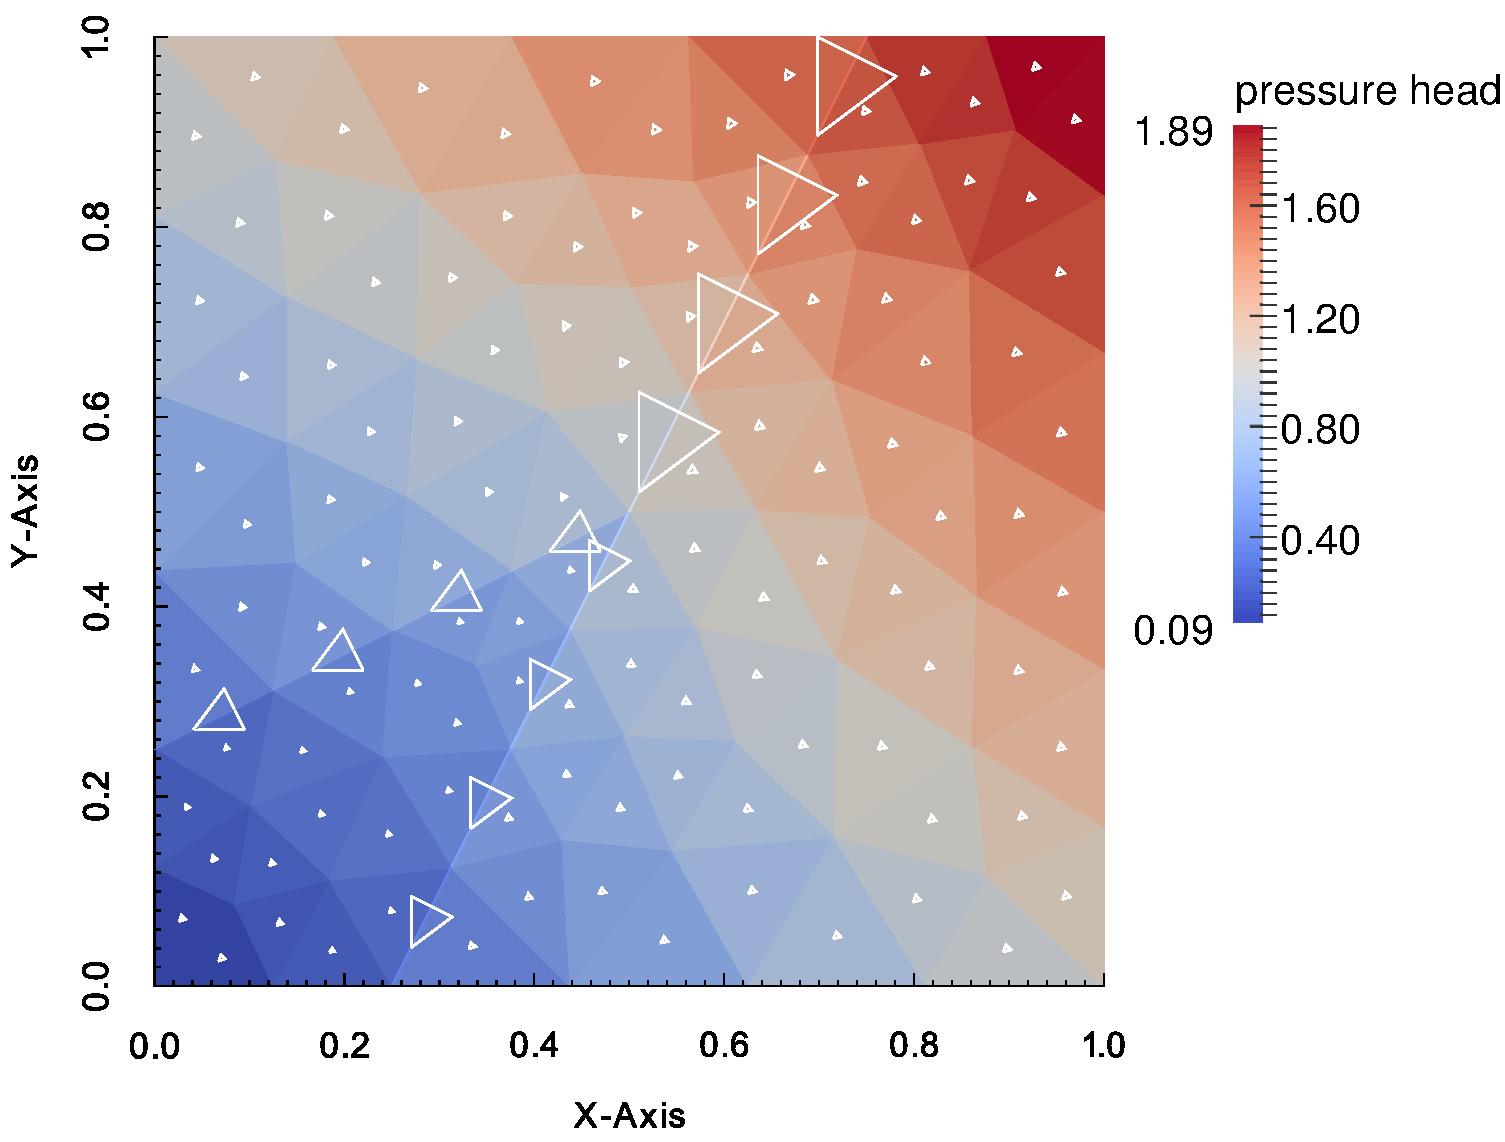
\includegraphics[width=\textwidth]{\fig/03_flow.pdf}
        % 03_flow.pdf: no raster
        \caption{Elementwise pressure head and\\velocity field denoted by triangles.\\ (Steady flow.)}
        \label{fig:tut-flow}
    \end{subfigure}
    ~
    \begin{subfigure}[b]{0.48\textwidth}
        \centering
        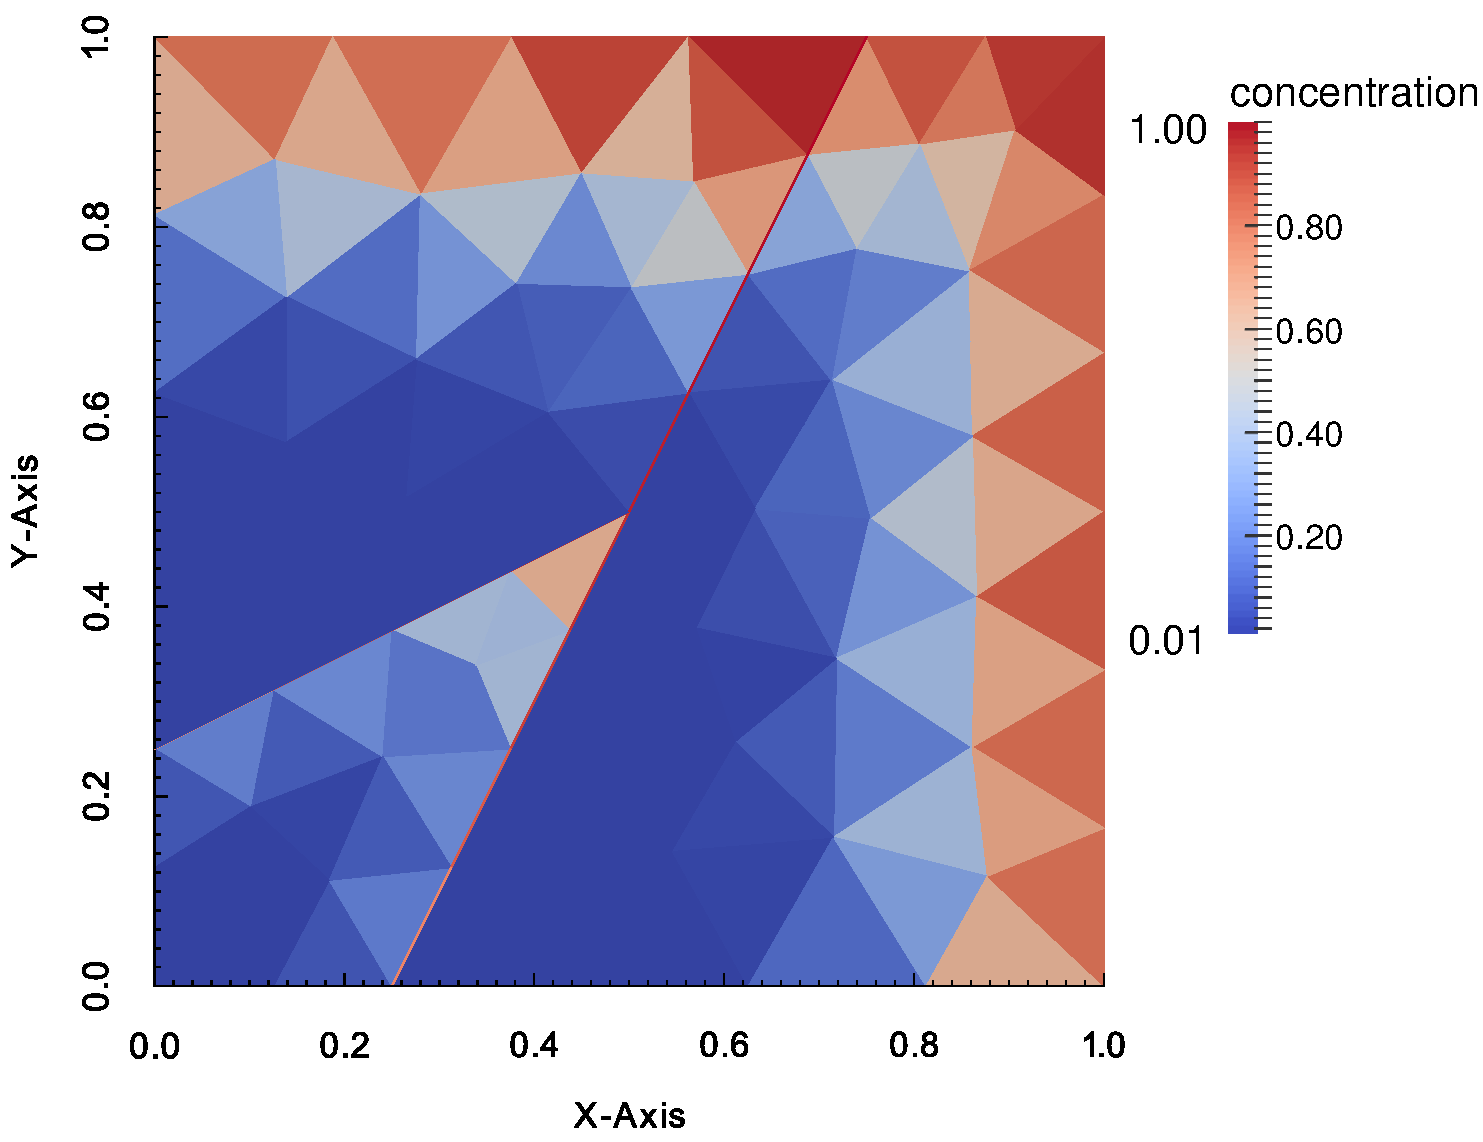
\includegraphics[width=\textwidth]{\fig/03_trans.pdf}
        % 03_trans.pdf: no raster
        \caption{Propagation of U235 from the inflow part of the boundary. \\ (At the time $9\cdot10^{5}$ s.)}
        \label{fig:tut-trans}
    \end{subfigure}
    \caption{Results of the tutorial problem.}
    \label{fig:tutorial}
\end{figure}
